\chapter{Test of Signal to Noise Ratio}

The test of SNR of the guitar is going to be presented in this appendix. It will include the used material and setup, the test procedure and the results. \\

\section{Material and Setup}

In order to perform this test, the following material has been used:

\begin{itemize}
	\item Electric guitar used during the project (same for all tests)
	\item Analog Discovery Digilent 2 USB Oscilloscope
	\item A computer with Waveforms 2015 and MATLAB
	\item Wires
\end{itemize}


The first step is to connect the oscilloscope to the computer with a USB cable and then connect the oscilloscope to the guitar. Different converters maybe needed. The user should ensure that none of the connections are loose in order to obtain the best results possible. \\

\section{Test Procedure}

The test is done in two steps. First, noise is measured without the guitar connected. It is done by measuring the maximum and the minimum amplitude of the signal of the ocilloscope alone. \\

The second test to make is to measure the noise with the guitar connected by taking the maximum and the minimum amplitude of the signal with the guitar connected.  \\

For each of the tests, a difference between the maximum and the minimum is made. The wanted value is the difference between the two resulting calculations. \\

\section{Results}

The plot of the signal amplitude without the guitar is shown in figure \ref{fig:without_guitar}. \\

\begin{figure}[hbt]
  \centering
  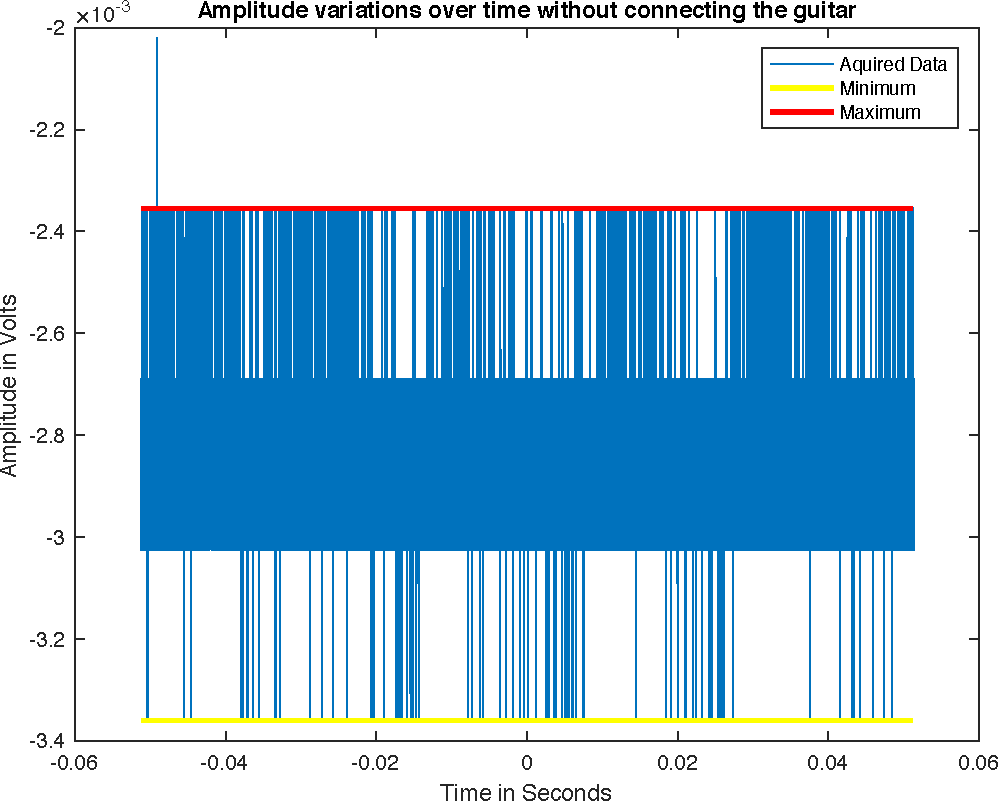
\includegraphics[width=1\textwidth]{without_guitar}
  \caption{Signal Amplitude without the guitar connected}
  \label{fig:without_guitar}
\end{figure}

The maximum value obtained is -0.002355 V and the minimum is -0.0034 V which gives a difference of 0.001045 V. \\

The plot of the signal amplitude with the guitar is shown in figure \ref{fig:with_guitar}. \\

\begin{figure}[hbt]
  \centering
  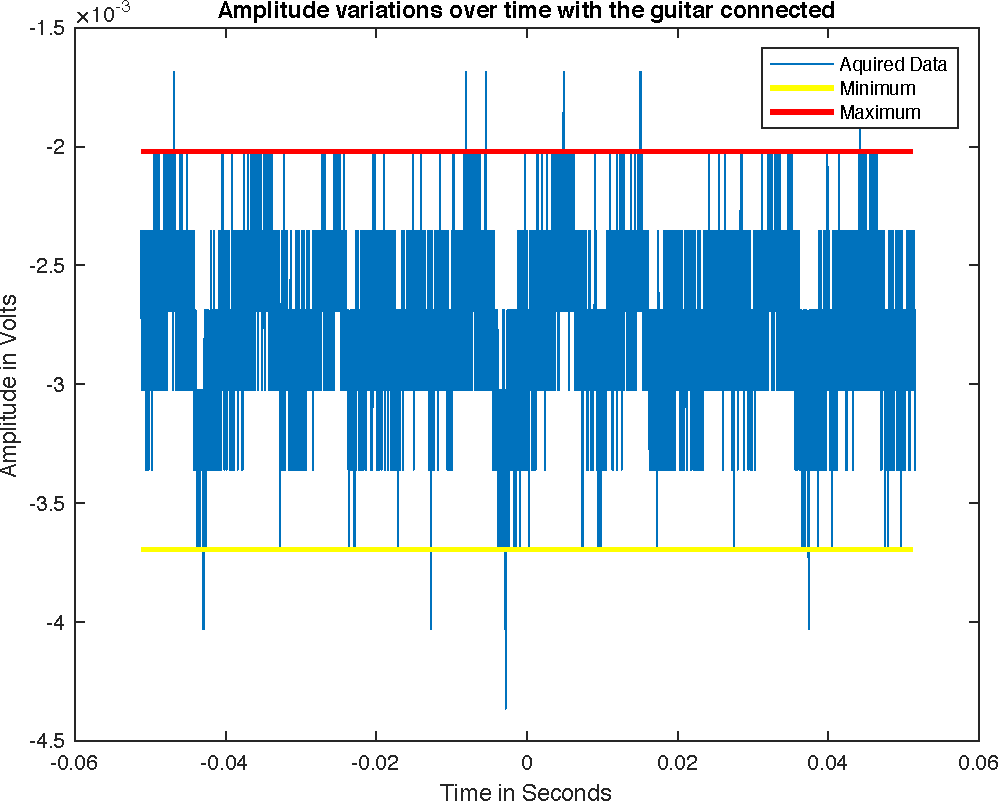
\includegraphics[width=1\textwidth]{with_guitar}
  \caption{Signal Amplitude without the guitar connected}
  \label{fig:with_guitar}
\end{figure}

The maximum and the minimum obtained from the aquired data seems to be -0.003693 V and -0.00202 V respectively which gives a difference of 0.001673 V.  \\
The difference between the two (max-min) is then 0.000628 V. \\
Supposing that the maximum signal that can be obtained peak to peak from the guitar is 2 V according to the test in \autoref{app:guitar_max_amplitude}, the signal to noise ratio is then:

\begin{equation}
	SNR = 20 \cdot log_{10}(\frac{2}{0.000628} = 70.06dB
	\end{equation}

Where:

$SNR$ is the signal to noise ratio of the guitar in dB \\


This result is subject to many errors. From the graphs in the two cases, it can be seen that the oscilloscope precision is not enough to get a clear conclusion. The sure conclusion is that the noise is of the order of 0.0001V but the exact value cannot be verified. In all cases, an SNR of the order 70dB can be assumed sufficient.